\documentclass[a4paper]{article}

\usepackage[romanian]{babel}
\usepackage{amsmath}
\usepackage{amssymb}
\usepackage{csquotes}
\usepackage{fontspec}
\usepackage{graphicx}

\usepackage[ruled]{algorithm2e}
\usepackage{minted}
\usemintedstyle{emacs}

\usepackage[backend=biber]{biblatex}
\addbibresource{main.bib}

\usepackage{geometry}
\geometry{
  top=3.5cm,
  bottom=3.5cm,
  left=3.5cm,
  right=3.5cm,
}

\usepackage{hyperref}
\hypersetup{
    colorlinks,
    citecolor=black,
    filecolor=black,
    linkcolor=black,
    urlcolor=black
}

\usepackage{tikz}
\usetikzlibrary{decorations.pathreplacing}

\newcommand\MemoryLayout[1]{
  \begin{tikzpicture}[scale=0.3]
     \foreach \pt/\lbl/\col/\lab [remember=\pt as \tp (initially 0)] in {#1} {
       \draw[thick](\pt,0)--++(0,3)node[above]{$\lbl$};
       \foreach \a [parse=true] in {\tp,...,\pt-1} {
          \draw[fill=\col](\a,0) rectangle ++(1,2);
       }
       \if\lab\relax\relax\else
         \draw[thick,decorate, decoration={brace,amplitude=4mm}]
            (\pt,-0.2)--node[below=4mm]{\lab} (\tp,-0.2);
       \fi
     }
     \draw[thick](0,0)--++(0,3)node[above]{$0$};
  \end{tikzpicture}
}

\SetKwInput{KwData}{Date}
\SetKwInput{KwResult}{Rezultat}
\SetKwInput{KwIn}{Intrare}
\SetKwInput{KwOut}{Ieșire}
\SetKw{KwTo}{pânâ la}
\SetKw{KwRet}{returnează}
\SetKw{Return}{returnează}
\SetKwBlock{Begin}{începe}{sfârșit}
\SetKwComment{tcc}{/*}{*/}
\SetKwComment{tcp}{//}{}
\SetKwIF{If}{ElseIf}{Else}{dacă}{atunci}{altfel dacă}{altfel}{sfârșit}
\SetKwSwitch{Switch}{Case}{Other}{comută}{execută}{caz}{altfel}{sfârșit}{sfârșit}
\SetKwFor{For}{pentru}{execută}{sfârșit}
\SetKwFor{While}{cât timp}{execută}{sfârșit}
\SetKwFor{ForEach}{pentru fiecare}{execută}{sfârșit}
\SetKwRepeat{Repeat}{repetă}{până când}
\SetAlgorithmName{Algoritm}{}{}

\begin{document}
\begin{titlepage}
	\begin{center}
		\Large Proiect pentru obținerea atestării profesionale în informatică
		\vfill
		\LARGE\textbf{Octarou: Interpretor pentru limbajul de programare \texttt{CHIP-8}}

		\vspace{8pt}
		\Large Nicolas-Ștefan Bratoveanu \\
		\large Prof. coordonator Mihaela Stan

		\vfill
		\Large
		Colegiul Național „Vasile Alecsandri” Galați \\
		2023-2024
	\end{center}
\end{titlepage}
\shipout\null

\tableofcontents
\newpage

%--------------------------------------------------------------------------------------------------------------------------------------------------------------%
\section{Introducere}
\subsection{Contextualizare}
\textit{Octarou} este un interpretor pentru limbajul de programare \texttt{CHIP-8}. Acesta este un limbaj de programare interpretat, dezvoltat
de către Joseph Weisbecker în 1977 pentru sisteme bazate pe microprocesorul RCA 1802. A fost inițial utilizată pe computerele COSMAC VIP și Telmac
1800. Limbajul a fost creat cu scopul de a permite dezvoltarea mult mai ușoară a jocurilor video pe aceste platforme, permițând utilizarea unor
instrucțiuni hexazecimale, în locul instrucțiunilor native \cite{langhoff}. Spre sfârșitul anilor '70, în spatele acestui limbaj se formase o comunitate activă
de dezvoltatori și utilizatori, care a luat naștere odată cu buletinul informativ \textit{VIPer} al revistei \textit{ARESCO}, ale cărei prime
ediții au dezvăluit codul pentru interpretorul original de \texttt{CHIP-8}.

CHIP-8 s-a răspândit pe alte platforme, precum computerele australiene DREAM 6800, ETI-660 și MicroBee, computerul finlandez menționat mai devreme,
Telmac 1800 și computerul canadian ACE VDU \cite{langhoff}.

Ulterior, au apărut interpretoare derivate și extensii la limbajul original, folosite, spre exemplu, pe calculatoare grafice (\texttt{CHIP-48}, \texttt{SUPER-CHIP}
pentru calculatoarele HP-48 \cite{langhoff}). Aceste dispozitive aparțineau perioadei de după anii '80 și aveau, de regulă, mult mai multă putere de procesare
decât microcomputerele din deceniul precedent, cum ar fi COSMAC VIP-ul.

\subsection{Motivația alegerii temei}
La nivel de suprafață, alegerea acestei teme poate părea (cel puțin) dubioasă. Cu toate că este, într-adevăr, o temă destul de obscură, consider
că este extrem de valoroasă. Astfel de proiecte au valoare din punct de vedere al istoriei calculatoarelor, precum și în cadrul fenomenului de
„retro-computing”. Mai mult decât atât, CHIP-8, în mod specific, are o valoare educațională deosebită, întrucât implementarea unui astfel de
sistem este adesea recomandată ca prim pas în lumea dezvoltării de emulatoare \cite{langhoff}.

%--------------------------------------------------------------------------------------------------------------------------------------------------------------%

\section{Mediul de dezvoltare}
\subsection{Rust}
Am ales Rust ca limbaj principal de dezvoltare pentru acest proiect. Rust este un limbaj de programare general, multi-paradigmă, care pune accent
pe siguranță, eficiență și paralelism. Este utilizat în numeroase situații, de la programarea sistemelor, la dezvoltarea de aplicații grafice, dezvoltarea
web sau a sistemelor integrate.

Performanța și eficiența se datorează absenței unui runtime și a unui \textit{garbage collector}. Siguranța memoriei este asigurată de către sistemul
de tipuri bogat și de modelul de \textit{ownership}, care permit eliminarea a numeroase tipuri de buguri în stagiul de compilare \cite{rsorg}. Modelul
de \textit{ownership} impune niște reguli privitoare la deținători \cite[Cap.~4.1]{rustbook}:
\begin{itemize}
	\item Orice valoare are un deținător (\textit{owner}).
	\item Nu poate exista decât un deținător la un moment dat.
	\item Când deținătorul iese din scope, valoarea este eliberată.
\end{itemize}
și la utilizarea referințelor \cite[Cap.~4.2]{rustbook}:
\begin{itemize}
	\item Referințele sunt mereu valide.
	\item La un moment dat, pot exista fie mai multe referințe imuabile, fie o singură referință muabilă, dar niciodată ambele.
\end{itemize}

Sistemul de tipuri este extrem de puternic și permite modelarea stării unei aplicații în moduri idiomatice, prin utilizarea tipurilor
pentru a impune invariantele. Spre exemplu, considerăm tipul de date din Listing~\ref{listing:nonzerou8}. Invarianta acestuia este
că valoarea pe care o memorează este diferită de 0. Acest lucru este reprezentat direct în sistemul de tipuri prin utilizarea
\texttt{Option<T>} (echivalent cu \texttt{Maybe a} din Haskell sau \texttt{std::optional<T>} din C++17), un tip polimorfic utilizat
pentru a încapsula o valoare sau \textit{absența acesteia}. Dacă valoarea pe care o primește constructorul \texttt{new} este nulă,
acesta va întoarce valoarea \texttt{None}, pe care apelatorul este forțat să o gestioneze.

\begin{listing}
	\inputminted{rust}{codeblocks/nonzerou8.rs}
	\caption{Exemplu de structură cu invariantă simplă}
	\label{listing:nonzerou8}
\end{listing}

Dacă se încearcă utilizarea valorii de tip \texttt{Option<u8>} ca atare, se obține o eroare de compilare.

\begin{minted}{rust}
let a = NonZeroU8::new(0);
println!("{:?}", a + 2);
\end{minted}
\begin{verbatim}
error[E0369]: cannot add `{integer}` to `Option<NonZeroU8>`
  --> src/main.rs:15:24
   |
15 |     println!("{:?}", a + 2);
   |                      - ^ - {integer}
   |                      |
   |                      Option<NonZeroU8>
\end{verbatim}

„Capturarea” erorilor în stagiul de compilare este una dintre super-puterile acestui limbaj.

\subsubsection{Librăriile \texttt{eframe} și \texttt{egui}}
\textbf{Egui} este o librărie simplă, rapidă și portabilă de tip \textit{immediate mode GUI} scrisă în Rust pur \cite{egui}, iar
\textbf{eframe} este o librărie utilizată alături de egui care pune la dispoziție interacțiunea dintre aceasta și platforma specifică
pe care o țintește aplicația (în cazul acesta, Windows, macOS, Linux, BSD și, parțial, WebAssembly). Spre deosebire de alte librării
de UI de tip \textit{retained mode}, folsind egui, aplicația redesenează procedural UI-ul în fiecare cadru. Am ales acest mediu
grafic pentru simplitate și, totodată, datorită faptului că aceste librării sunt scrise în întregime în Rust și beneficiază, prin urmare
de avantajele de securitate, corectitudine și performanță asociate.

\subsection{Nix}
Nix este un gestionar de pachete pentru sisteme Unix-like bazat pe un \textit{model pur funcțional de implementare a software-ului} \cite{edolstra}.
Acesta gestionează problema implementării și distribuirii pachetelor de software prin instalarea lor într-o locație centralizată, în directoare
unice, discriminate printr-un hash criptografic. Astfel, elimină problemele asociate lipsei de dependențe și permite coexistența mai multor
versiuni ale aceluiași pachet (aici, versiune nu se referă doar la numărul de versiune semantică, ci include și parametrii procesului de compilare
a pachetului).

\textit{Octarou} se bazează pe un Nix flake atât în procesul de dezvoltare cât și în cel de compilare și distribuție. Fișierul \texttt{flake.nix} conține
o descriere declarativă (\textit{derivație}) a procesului de compilare al aplicației (Listing~\ref{listing:nix-native-build}), dar și a shellului utilizat
pentru dezvoltarea acesteia. Pentru aceasta am
utilizat librăria \textit{Crane}\footnote{O librărie Nix pentru compilarea proiectelor Rust prin Cargo. (https://crane.dev/)}, care facilitează
descărcarea dependințelor (versiuni fixe, declarate în \texttt{flake.lock}) și compilare incrementală și compozabilă.

Pachetele Nix sunt definite cu ajutorul unui limbaj funcțional cu evaluare leneșă concepută special pentru gestionarea pachetelor. Dependințele
sunt urmărite folosind un format intermediar (\textit{derivațiile}), care se află, alături de restul pachetelor, într-o locație centralizată numită
\textit{Nix store} (de obicei, la \texttt{/nix/store}). Derivațiile și specificațiile derivațiilor din Nix store sunt eliminate automat prin
\textit{garbage collection}. Acest model funcțional garantează că orice actualizare a pachetelor este \textit{atomică} și permite rollback-uri
în timp constant $\mathcal{O}(1)$ \cite{edolstra}.

Repozitoriul principal în care se poate găsi întreaga colecție de pachete ce pot fi distribuite prin Nix se numește \href{https://github.com/nixos/nixpkgs}{\texttt{nixpkgs}}.
Acesta găzduiește și codul-sursă pentru NixOS, o distribuție de Linux bazată pe gestionarul de pachete Nix, care este întru totul configurabilă prin
limbajul Nix.

\begin{listing}
	\inputminted{nix}{codeblocks/package.nix}
	\caption{Derivația procesului de compilare pe platforma nativă}
	\label{listing:nix-native-build}
\end{listing}

\begin{listing}
	\inputminted{nix}{codeblocks/cross.nix}
	\caption{Toolchainul utilizat pentru cross-compilare pentru Windows}
	\label{listing:nix-cross-build}
\end{listing}

\subsubsection{Cross-compilare}
Pachetele pentru \texttt{x86\_64-pc-windows-gnu} sunt compilate prin Nix și Crane, folosind facilitățile de cross-compilare (Listing~\ref{listing:nix-cross-build})
din \texttt{nixpkgs}. Procesul acesta este declanșat automat printr-un pipeline de CI pentru fiecare versiune semantică a proiectului. Un
mecanism similar este utilizat pentru compilarea pentru \texttt{wasm32-unknown-unknown}, arhitectura-țintă pentru platforma web\footnote{
	WebAssembly încă nu susține toate API-urile utilizate în logica interpretorului (\texttt{std::time::Instant}),
	motiv pentru care, pe această platformă, aplicația se comportă în moduri non-ideale.}.

% \begin{listing}[hbt!]
% 	\inputminted{nix}{codeblocks/paper.nix}
% 	\caption{Derivația acestui document \LaTeX}
% \end{listing}

%--------------------------------------------------------------------------------------------------------------------------------------------------------------%

\begin{table}
	\begin{center}
		\begin{tabular}{ |p{5em}|p{8em}|p{16em}| }
			\hline
			\textbf{Componentă} & \textbf{Mărime}                       & \textbf{Utilizare}                                                                                             \\
			\hline\hline
			Memorie             & 4 KB, adrese pe 16 biți               & Memorie volatilă                                                                                               \\
			\hline
			Display             & 64x32 pixeli                          & Grafică                                                                                                        \\
			\hline
			Stivă               & practic nelimitată, adrese pe 16 biți & Structură de tip LIFO; utilizată pentru apelarea subprogramelor                                                \\
			\hline
			Delay               & 8 biți                                & Decrementat cu o frecvență de 60 Hz; utilizat pentru calculul timpilor în aplicații                            \\
			\hline
			Sound               & 8 biți                                & Decrementat la fel ca Delay; utilizat pentru gestionarea sunetelor                                             \\
			\hline
			Index               & 16 biți                               & Registru utilizat pentru a indexa memoria (pentru sprite-uri, font etc.)                                       \\
			\hline
			Program Counter     & 16 biți                               & Registru care indică adresa de memorie a instrucțiunii ce urmează să fie executată                             \\
			\hline
			Variables           & 16 registre de 8 biți                 & Sunt numerotate de la V0 la VF (hexazecimal); folosite ca variabile; VF este folosit ca \textit{flag register} \\
			\hline
		\end{tabular}
		\caption{Componentele interpretorului \texttt{CHIP-8} \cite{langhoff}}
		\label{tab:componente}
	\end{center}
\end{table}

%--------------------------------------------------------------------------------------------------------------------------------------------------------------%

\section{Funcționarea \texttt{CHIP-8}}
Interpretorul \texttt{CHIP-8} operează pe componentele enumerate în Tabela~\ref{tab:componente}, citind instrucțiuni din memorie și executându-le,
modificând memoria și registrele corespunzător.

\subsection{Instrucțiunile}
Instrucțiunile \texttt{CHIP-8} sunt reprezentate prin numere de 16 biți, citite din memorie, de la adresa indicată de program counter. Simbolic,
acestea se reprezintă prin 4 cifre hexazecimale. Primii 4 biți (primul \textit{nibble}) discriminează categoriile de instrucțiuni.

Majoritatea instrucțiunilor au una din formele următoare. Cu toate că valorile din cadrul codului instrucțiunii sunt mai mici de 8 sau 16 biți, ele
sunt tratate ca valori de 8 respectiv 16 biți. În implementația aceasta, valorile de 16 biți sunt tratate ca \texttt{usize}, deoarece sunt folosite
pentru a indexa tablouri.
\begin{itemize}
	\item \texttt{00EE} -- formă literală; o valoare fixă
	\item \texttt{0NNN} -- formă parametrică; \texttt{NNN} reprezintă o valoare pe 16 biți (de obicei o adresă de memorie)
	\item \texttt{0XNN} -- formă parametrică; \texttt{X} reprezintă o valoare pe 8 biți (de obicei indexul unui registru de variabile), iar \texttt{NN}, o valoare pe 16 biți (de obicei o adresă de memorie)
	\item \texttt{0XYN} -- formă parametrică; \texttt{X} și \texttt{Y} reprezintă indecși pentru registrele de variabile, iar \texttt{N}, o valoare pe 8 biți
\end{itemize}

\begin{listing}[ht!]
	\inputminted{rust}{codeblocks/opcodes.rs}
	\caption{Funcțiile utilizate pentru parsarea codurilor de instrucțiuni}
	\label{listing:xyn}
\end{listing}

\pagebreak

\subsection{Memoria}
Memoria are în total 4 KB, adică $2^{12} = 4096$ de octeți. Acest spațiu este adresabil cu adrese de 12 biți, însă, în practică, se folosesc adrese de 16 biți.
Spre exemplu, registrul \textit{index} (\texttt{I}) reține o adresă de 16 biți care indică locația din memorie a sprite-urilor ce trebuie desenate pe ecran.

Pe COSMAC VIP, zona de memorie dintre 0 și 512 biți era ocupată de codul interpretorului (din pricina limitațiilor
tehnice), însă în cazul interpretoarelor moderne, acest lucru nu este necesar; memoria aceea este utilizată, în schimb,
pentru stocarea fontului, care se pune, de regulă, în zona 80--160 biți (Figura~\ref{figure:memory}).

\begin{figure}[hbt!]
	\begin{center}
		\MemoryLayout{
		10/512b/blue!20/{Interpretorul},
		40/4096b/white/{Programul \texttt{CHIP-8}}
		}
		\MemoryLayout{
		2/80b/gray!20/{Gol},
		6/160b/green!20/{Font},
		10/512b/gray!20/{Gol},
		40/4096b/white/{Programul \texttt{CHIP-8}}
		}
		\caption{Layoutul de memorie \texttt{CHIP-8} (\underline{NU} la scară)}
		\label{figure:memory}
	\end{center}
\end{figure}

Toată memoria este modificabilă, iar programele interpretate se pot și se vor modifica pe ele însele \cite{langhoff}.

\subsubsection{\texttt{ANNN, FX1E} și \texttt{FX29}}
Toate aceste instrucțiuni manipulează registrul \texttt{I}. \texttt{ANNN} (\textit{SetIndex}) pur și simplu setează $\texttt{I} \gets \texttt{NNN}$, iar
\texttt{FX1E} (\textit{AddIndex}) adaugă \texttt{VX} la \texttt{I} ($\texttt{I} \gets \texttt{I} + \texttt{NNN}$).
Instrucțiunea \texttt{FX29} se numește \textit{SetIndexFont} și setează \texttt{I} la adresa din memorie a caracterului reprezentat de ultimii 4 biți
(ultimul \textit{nibble}) ai valorii din \texttt{VX}.

\subsubsection{\texttt{FX55} și \texttt{FX65}}
Aceste instrucțiuni sunt folosite pentru stocarea și citirea din memorie a valorilor din registrele variabile. \textit{StoreMemory}, \texttt{FX55},
scrie succesiv în memorie, începând de la adresa \texttt{I}, valorile din registrele \texttt{V0} până la \texttt{VX}. \textit{LoadMemory}, \texttt{FX65}
face opusul: citește din memorie, începând de la adresa \texttt{I}, valorile din registrele \texttt{V0}--\texttt{VX}.

În interpretorul de pe COSMAC VIP, această instrucțiune incrementa valoarea din \texttt{I}, astfel încât la finalul execuției instrucțiunii aceasta memora
valoarea $\texttt{I} + \texttt{X} + 1$. Interpretoarele moderne (de la \texttt{CHIP-48} și \texttt{SUPER-CHIP} înainte) nu fac acest lucru; valoarea indexului
rămâne neschimbată \cite{langhoff}\cite{gulrak}.

\subsection{Ecranul, sprite-urile și fontul}
Ecranul este actualizat cu o rată de 60 Hz. Fiecare pixel este fie pornit fie oprit.

Un sprite este o secvență de octeți cu lungimea $1 \leq n \leq 15$. Fiecare octet reprezintă un „rând”, iar fiecare bit din octet reprezintă
un pixel. Instrucțiunea care desenează sprite-uri pe ecran este \texttt{DXYN} și va fi detaliată mai târziu, însă, pe scurt, ea efectuează o operațiune
analoagă disjuncției logice exclusive (\textit{exclusive or}) între fiecare pixel al sprite-ului și cel corespunzător de pe ecran \cite{langhoff}.

Fontul este alcătuit din 16 sprite-uri de 4x5 pixeli care reprezintă cifrele hexazecimale 0--F. Caracterele sunt desenate pe ecran la fel ca
sprite-urile obișnuite \cite{langhoff}.

\subsubsection{\texttt{00E0} și \texttt{DXYN}}
Instrucțiunea \texttt{00E0} (\textit{Clear}) resetează ecranul, adică setează toți pixelii la valoarea 0.

Instrucțiunea \texttt{DXYN} (\textit{Draw}) este mai complexă. Aici, \texttt{X} și \texttt{Y} reprezintă registrele variabile care conțin coordonatele
de pe ecran la care trebuie desenat sprite-ul indicat de registrul \texttt{I} (\textit{index}), iar \texttt{N} reprezintă înălțimea sprite-ului
care trebuie desenat. Cu alte cuvinte, trebuie desenat pe ecran sprite-ul din zona de memorie \texttt{I..I+N}, la coordonatele VX, respectiv,
VY~\footnote{În implementarea acestei instrucțiuni, valoarea registrului \texttt{I} nu este modificată în niciun fel.}. Coordonatele din VX și VY
sunt reduse modulo 64, respectiv, 32, adică se „învârt” după marginile ecranului. În schimb, dacă sprite-ul depășește marginile ecranului, acesta
este pur și simplu tăiat.

\begin{algorithm}[hbt!]
	\caption{Desenarea unui sprite}\label{alg:dxyn}
	\tcp{Coordonatele inițiale se „învârt” în jurul ecranului}
	$x\gets$ VX$\mod 64$\;
	$y\gets$ VY$\mod 32$\;
	VF $\gets 0$\;
	\For{$dy\gets 0,N-1$}{
		\For{$dx\gets 0,7$}{
			\tcp{Sprite-ul este tăiat la marginile ecranului}
			\If{$y + dy < 32$ și $x + dx < 64$}{
				\tcp{$D$ este un tablou bidimensional ce reprezintă ecranul}
				\tcp{$M$ este un tablou ce reprezintă memoria}
				$b \gets$ al $dx$-lea bit din $M[I + dy]$\;
				VF $\gets b \land D[y + dy][x + dx]$\;
				$D[y + dy][x + dx] \gets b \oplus D[y + dy][x + dx]$\;
			}
		}
	}
\end{algorithm}

Pentru fiecare pixel din sprite, acesta modifică pixelul de pe ecran cu care se suprapune prin operația de disjuncție exclusivă. Dacă vreun pixel
de pe ecran a fost dezactivat (setat la 0) de această instrucțiune, atunci se setează VF la 1, altfel, VF este setat la 0 \cite{langhoff}.
Algoritmul~\ref{alg:dxyn} reprezintă în linii mari, în pseudocod, procesul de desenare a unui sprite pe ecran.

\subsection{Controlul fluxului și apelarea subprogramelor}
Controlul fluxului se realizează printr-o serie de instrucțiuni de tip \textit{jump} sau \textit{skip}.

\subsubsection{\texttt{1NNN} și \texttt{BNNN}/\texttt{BXNN}}
Instrucțiunile \texttt{1NNN} (\textit{Jump}) și \texttt{BNNN} (\textit{JumpOffset}) sunt utilizate pentru a seta program counterul la o adresă
de memorie specifică. \textit{Jump} setează \texttt{PC} la adresa \texttt{NNN}. \textit{JumpOffset} este mai ambiguă \cite{langhoff}. În interpretorul
original de \texttt{CHIP-8}, această instrucțiune sărea la adresa $\texttt{NNN} + \texttt{V0}$. În \texttt{CHIP-48} și \texttt{SUPER-CHIP}, ea funcționează
ca \texttt{BXNN}, sărind la adresa $\texttt{XNN} + \texttt{VX}$.

\subsubsection{\texttt{3XNN, 4XNN, 5XY0} și \texttt{9XY0}}
Aceste instrucțiuni sar peste următoarea instrucțiune, adică incrementează \texttt{PC} cu 2, astfel:
\begin{itemize}
	\item \texttt{3XNN} va sări peste o instrucțiune dacă $\texttt{VX} = \texttt{NN}$.
	\item \texttt{4XNN} va sări peste o instrucțiune dacă $\texttt{VX} \not = \texttt{NN}$.
	\item \texttt{5XY0} va sări peste o instrucțiune dacă $\texttt{VX} = \texttt{VY}$.
	\item \texttt{9XY0} va sări peste o instrucțiune dacă $\texttt{VX} \not = \texttt{VY}$.
\end{itemize}

Combinându-le cu instrucțiunile \textit{jump}, se poate obține un mecanism de control al fluxului similar cu \texttt{if}-ul din limbajele de programare moderne.

\subsubsection{\texttt{00EE} și \texttt{2NNN}}
Subprogramele funcționează într-un mod similar cu Assembly. Instrucțiunea \texttt{2NNN} (\textit{Call}) stochează adresa indicată de program counter (\texttt{PC})
în stiva de apel, iar apoi setează \texttt{PC}-ul la o altă adresă. Instrucțiunea \texttt{00EE} (\textit{Return}) scoate o adresă din stivă și setează \texttt{PC}-ul
la acea adresă \cite{langhoff}.

\subsection{Tastatura}
Calculatoarele pe care \texttt{CHIP-8} obișnuia să ruleze utilizau tastaturi hexazecimale, cu 16 taste, de regulă dispuse într-o grilă de 4x4.
COSMAC VIP și calculatoarele HP48 utilizau dispunerea tastaturii din Figura~\ref{fig:keypad}, pe care o implementează și \textit{Octarou}.

\begin{figure}
	\begin{center}
		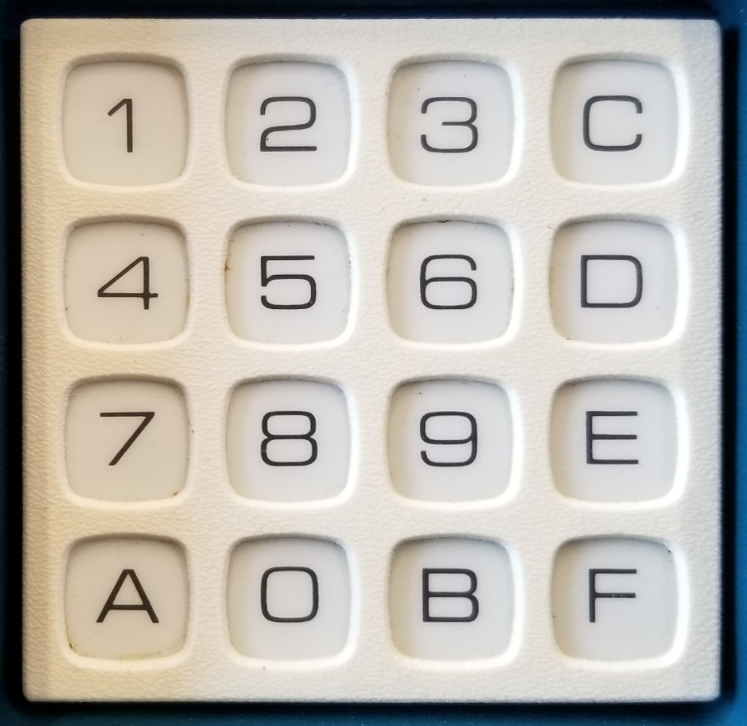
\includegraphics[width=0.6\textwidth]{figures/cosmac-vip-keypad.png}
	\end{center}
	\caption{Tastatura de pe COSMAC VIP}
	\label{fig:keypad}
\end{figure}

\subsubsection{\texttt{EX9E, EXA1} și \texttt{FX0A}}
Primele două instrucțiuni sunt de tip \textit{skip} și sar peste instrucțiuni în funcție de tastele apăsate, fără să aștepte apăsarea unei taste.
\begin{itemize}
	\item \texttt{EX9E} sare peste următoarea instrucțiune dacă tasta corespunzătoare valorii din \texttt{VX} este apăsată.
	\item \texttt{EXA1} sare peste următoarea instrucțiune dacă tasta corespunzătoare valorii din \texttt{VX} \underline{NU} este apăsată.
\end{itemize}

Cea de-a treia, \texttt{FX0A}, oprește execuția instrucțiunilor (dar nu și decrementarea temporizatorilor) până ce o tastă este apăsată (și eliberată),
caz în care valoarea corespunzătoare tastei este pusă în \texttt{VX}.

\subsection{Temporizatoarele}
Cele două registre \texttt{delay} și \texttt{sound} funcționează în mod identic. Au mărimea de 1 octet, deci pot reprezenta valori până la 255.
Cât timp valorile lor sunt mai mari decât 0, ele sunt decrementate cu 1 de 60 de ori pe secundă, iar acest lucru se întâmplă independent
de bucla de execuție a instrucțiunilor.
Registrul \texttt{sound} cauzează un sunet cât timp valoarea sa este mai mare decât 0.

\subsubsection{\texttt{FX15, FX07} și \texttt{FX18}}
Aceste instrucțiuni se utilizează pentru a manipula registrele de temporizare. Instrucțiunea \texttt{FX15} (\textit{SetDelay}) setează registrul
\texttt{delay} la valoarea din \texttt{VX}, iar \texttt{FX18} (\textit{SetSound}) setează registrul \texttt{sound} la valoarea din \texttt{VX}.
\texttt{FX07} pune valoarea din \texttt{delay} în \texttt{VX}.

\subsection{Instrucțiunile aritmetice și logice}
Majoritatea instrucțiunilor aritmetice (Tabela~\ref{table:ops}) afectează registrul \texttt{VF}, excepție făcând \texttt{6XNN} și \texttt{7XNN}.

\subsubsection{\texttt{6XNN} și \texttt{7XNN}}
Ambele instrucțiuni manipulează registrele de variabile. \textit{SetLiteral} (\texttt{6XNN}) pur și simplu efectuează $\texttt{VX} \gets \texttt{NN}$.
\textit{AddLiteral} adună la registrul variabil o valoare ($\texttt{VX} \gets \texttt{VX} + \texttt{NN}$), fără a modifica valoarea din registrul flag
\texttt{VF}.

\begin{table}
	\centering
	\begin{tabular}{ |l|l|l|l| }
		\hline
		\textbf{Codul} & \textbf{Numele}     & \textbf{Operația}                                  & \textbf{Flag register}                                \\
		\hline
		\texttt{8XY0}  & \textit{Set}        & $\texttt{VX} \gets \texttt{VY}$                    &                                                       \\
		\hline
		\multicolumn{4}{|c|}{\textbf{Operații logice pe biți}}                                                                                            \\
		\hline
		\texttt{8XY1}  & \textit{Or}         & $\texttt{VX} \gets \texttt{VX} \lor   \texttt{VY}$ &                                                       \\
		\texttt{8XY2}  & \textit{And}        & $\texttt{VX} \gets \texttt{VX} \land  \texttt{VY}$ &                                                       \\
		\texttt{8XY3}  & \textit{Xor}        & $\texttt{VX} \gets \texttt{VX} \oplus \texttt{VY}$ &                                                       \\
		\texttt{8XY6}  & \textit{RightShift} & $\texttt{VX} \gets \texttt{VY} \ll 1$              & $\texttt{VF} \gets \texttt{VY} \land 1$               \\
		\texttt{8XYE}  & \textit{LeftShift}  & $\texttt{VX} \gets \texttt{VY} \gg 1$              & $\texttt{VF} \gets \texttt{VY} \gg 7$                 \\
		\hline
		\multicolumn{4}{|c|}{\textbf{Operații aritmetice}}                                                                                                \\
		\hline
		\texttt{8XY4}  & \textit{Add}        & $\texttt{VX} \gets \texttt{VX} + \texttt{VY}$      & $\texttt{VF} \gets (\texttt{VX} + \texttt{VY} > 255)$ \\
		\texttt{8XY5}  & \textit{Sub}        & $\texttt{VX} \gets \texttt{VX} - \texttt{VY}$      & $\texttt{VF} \gets (\texttt{VY} < \texttt{VX})$       \\
		\texttt{8XY7}  & \textit{Sub}        & $\texttt{VX} \gets \texttt{VY} - \texttt{VX}$      & $\texttt{VF} \gets (\texttt{VX} < \texttt{VY})$       \\
		\hline
	\end{tabular}
	\caption{Operațiile aritmetice \texttt{CHIP-8}}\label{table:ops}
\end{table}

\subsubsection{Registrul \texttt{VF}}
Instrucțiunea \textit{Add} setează \texttt{VF} la 1 daca valoarea maxima (255) este depășită. \textit{Sub} începe prin a seta \texttt{VF} la 1, iar apoi,
dacă scăzătorul este mai mare decât descăzutul, „împrumută” din \texttt{VF}, setându-l la 0.

Operațiile \textit{LeftShift} și \textit{RightShift} au comportamente diferite în funcție de varianta \texttt{CHIP-8}. Pe COSMAC VIP, \texttt{VX} lua valoarea
lui \texttt{VY}, apoi i se aplica operația de bitshift. Pe \texttt{CHIP-48} și \texttt{SUPER-CHIP}, \texttt{VY} este ignorat complet, operația aplicându-i-se
numai lui \texttt{VX}.

\subsection{Alte instrucțiuni}
Alte două instrucțiuni \texttt{CHIP-8} sunt \texttt{CXNN} (\textit{Random}) și \texttt{FX33} (\textit{DecimalConversion}).
\textit{Random} generează un număr aleator, apoi pune în \texttt{VX} conjuncția pe biți dintre numărul generat și \texttt{NN}.

\textit{DecimalConversion} ia numărul din \texttt{VX} (un număr de 8 biți, adică $0 \leq \texttt{VX} \leq 255$) și scrie în zona de memorie \texttt{I..I+3}
cele 3 cifre în baza 10 ale acestuia (Algoritmul~\ref{alg:base10}).

\begin{algorithm}
	\caption{Conversie în baza 10}\label{alg:base10}
	$n \gets \texttt{VX}$\;
	\For{$j \gets 3,0,-1$}{
		$M[I + j] \gets n \mod 10$\;
		$n \gets n / 10$\;
	}
\end{algorithm}

%--------------------------------------------------------------------------------------------------------------------------------------------------------------%

\section{Aplicația}
\textit{Octarou} are o structură modulară simplă. Repozitoriul principal conține:
\begin{itemize}
	\item fișierele de configurare ale mediului de dezvoltare (\texttt{flake.nix, Cargo.toml} etc.)
	\item codul sursă al aplicației, sub \texttt{src/}
	      \subitem modulul \texttt{interpreter}, unde se află implementațiile variantelor de \texttt{CHIP-8}
	      \subitem modulul \texttt{app}, unde se află codul pentru interfața grafică
	      \subitem modulul \texttt{main}, punctul de intrare al aplicației
	\item documentația, incluzând acest document și sursa \LaTeX, licența (\texttt{EUPL-1.2}) și instrucțiuni de compilare
	\item programe \texttt{CHIP-8} (ROMuri), sub \texttt{roms/}
	\item ROMuri pentru testarea interpretorului, sub \texttt{tests/}
\end{itemize}

State-ul aplicației există în structura \texttt{Octarou} (Listing~\ref{listing:app}). Câmpul \texttt{interpreter} are tipul
\texttt{Option<Box<dyn Interpreter>>}, un smart pointer (\texttt{Box<T>}) la un trait-object de tip \texttt{dyn Interpreter}.
Acesta este state-ul interpretorului. Interpretoarele sunt mereu asociate cu un program. Odată cu încărcarea unui program, un
nou astfel de obiect este creat, iar cel vechi este eliberat (dacă există). Totodată, pentru a putea susține mai multe variante
de \texttt{CHIP-8}, în cazul acesta \texttt{CHIP-8} și \texttt{SUPER-CHIP}, este utlizată o formă de polimorfism bazată pe traituri.

Traitul \texttt{Interpreter} (Listing~\ref{listing:trait}) este implementat de două alte tipuri, anume \texttt{Chip8} (Listing~\ref{listing:chip8struct})
și \texttt{SuperChip}, fiecare din ele implementând varianta corespunzătoare a limbajului \texttt{CHIP-8}. Orice tip care implementează traitul
\texttt{Interpreter} trebuie să implementeze toate funcțiile asociate acestuia, adică, cu alte cuvinte, orice timp „vrea să fie un interpretor
de \texttt{CHIP-8}” trebuie să aibă un display, sa își poată actualiza timerele, să citească și să execute o instrucțiune etc.

\begin{listing}[hbt!]
	\begin{center}
		\inputminted{rust}{codeblocks/app-struct.rs}
		\caption{State-ul aplicației}\label{listing:app}
	\end{center}
\end{listing}

\begin{listing}[hbt!]
	\begin{center}
		\inputminted{rust}{codeblocks/interpreter-trait.rs}
		\caption{Traitul \texttt{Interpreter}}\label{listing:trait}
	\end{center}
\end{listing}

\subsection{Interpretarea \texttt{CHIP-8}}
Un interpretor de \texttt{CHIP-8}, în principiu, execută trei pași într-o buclă infinită: citește o instrucțiune din memorie, decodează
instrucțiunea pentru a afla ce trebuie să facă, iar apoi execută instrucțiunea \cite{langhoff}. Exterior acestei bucle, temporizatoarele
trebuie actualizate cu rata de 60 Hz. Bucla de execuție trebuie executată și ea cu o anumită viteză, întrucât, dacă ar fi executată prea
repede, programele și jocurile \texttt{CHIP-8} ar fi greu sau imposibil de folosit. Prin urmare, ea rulează implicit de 700 de ori pe secundă,
însă aceast parametru poate fi modificat prin interfață grafică a aplicației.

\begin{listing}[hbt!]
	\begin{center}
		\inputminted{rust}{codeblocks/chip8.rs}
		\caption{Structura interpretorului de \texttt{CHIP-8}}\label{listing:chip8struct}
	\end{center}
\end{listing}

\begin{listing}[hbt!]
	\begin{center}
		\inputminted{rust}{codeblocks/next-instruction.rs}
		\caption{Funcția pentru citirea și decodarea instrucțiunilor}\label{listing:nextinst}
	\end{center}
\end{listing}

\subsubsection{Citirea și decodarea instrucțiunilor}
Citirea și decodarea instrucțiunilor se realizează cu ajutorul funcției \verb|next_instruction| (Listing~\ref{listing:nextinst}).
Ea este responsabilă pentru a extrage și interpreta instrucțiunile din memoria interpretorului \texttt{CHIP-8}. Aceasta începe
prin extragerea următorului opcode (cod operațional) din memoria sistemului, interpretând 2 octeți (16 biți) de la adresa curentă a programului.
Apoi, avansând adresa programului cu 2 pentru a indica următoarea instrucțiune, funcția încearcă să creeze o nouă instrucțiune Chip8 folosind
opcode-ul extras. În cazul în care opcode-ul este necunoscut sau adresa indicată depășește memoria disponibilă, funcția returnează varianta
\texttt{Err} a tipului \verb|Result<Instruction, InterpreterError>|.

Tipul \texttt{Instruction} este o enumerație (un tip de date algebric) care memorează diferitele tipuri de instrucțiune. Semnătura funcției
care parsează codul operațional este

\mint{rust}|pub fn new(opcode: u16) -> Option<Self>|

În cazul în care primește un cod invalid, aceasta va întoarce varianta \verb|None|, care va semnifica apelatorului că nu există o instrucțiune
asociată acelui cod.

\subsubsection{Executarea instrucțiunilor}
Funcția \verb|execute_instruction| este responsabilă pentru executarea instrucțiunilor interpretate din memoria interpretorului \texttt{CHIP-8}.
Aceasta primește o instrucțiune și starea curentă a tastelor, apoi, în funcție de tipul instrucțiunii, efectuează operațiile corespunzătoare.

\subsection{Extensia \texttt{SUPER-CHIP}}
În anul 1990, Erik Bryntse a scris un emulator \texttt{Chip8} pentru calculatorul grafic HP-48 numit \texttt{CHIP-48}, care adaugă o serie
de instrucțiuni extinse denumite \texttt{SCHIP} sau \texttt{SUPER-CHIP}. \texttt{SUPER-CHIP} își propune să fie compatibil cu versiunea obișnuită
a setului de instrucțiuni \texttt{Chip8}, iar noile instrucțiuni ocupă spațiul neutilizat din codificarea instrucțiunilor \texttt{Chip8} \cite{bryntse}.

\textit{Octarou} implementează \texttt{SUPER-CHIP} și folosește polimorfismul pentru a permite încărcarea dinamică a programelor într-un interpretor
de \texttt{SUPER-CHIP}.

În ceea ce privește noutățile aduse de \texttt{SUPER-CHIP} față de \texttt{CHIP-8}, există mai multe îmbunătățiri și extinderi ale setului de instrucțiuni.
În primul rând, \texttt{SUPER-CHIP} adaugă un ecran mai mare, de dimensiuni 128x64 pixeli, față de ecranul de 64x32 pixeli al \texttt{CHIP-8}. De asemenea,
\texttt{SUPER-CHIP} include un set suplimentar de instrucțiuni grafice, cum ar fi desenarea sprite-urilor mai mari, de dimensiuni de 16x16 pixeli.
Iată instrucțiunile noi adăugate în \texttt{SUPER-CHIP} \cite{chip8research}.

\begin{itemize}
	\item \texttt{00FF} (\verb|Hires|) -- Activează modul grafic de înaltă rezoluție 128x64.
	\item \texttt{00FE} (\verb|Lores|) -- Dezactivează modul grafic de înaltă rezoluție și revine la 64x32.
	\item \texttt{00CN} (\verb|ScrollDown {amount: usize}|) -- Derulează ecranul în jos cu 0 până la 15 pixeli.
	\item \texttt{00FB} (\verb|ScrollRight|) -- Derulează ecranul la dreapta cu 4 pixeli.
	\item \texttt{00FC} (\verb|ScrollLeft|) -- Derulează ecranul la stânga cu 4 pixeli.
\end{itemize}

\begin{listing}
	\begin{center}
		\inputminted{rust}{codeblocks/scroll.rs}
		\caption{Implementația derulării pentru \texttt{SUPER-CHIP} în modul \texttt{hires}}
	\end{center}
\end{listing}

\subsection{Interfața grafică}
Interfață grafică este implementată prin librăriile \texttt{eframe} și \texttt{egui}. Este împărțită în două panouri: unul în stânga, unde se află
meniul și alte controale ale interpretorului, și unul principal, unde se află afișajul interpretorului. Ecranul principal găzduiește și o listă cu
mesaje de logging, accesabilă prin intermediul meniului cu taburi din partea de sus a ferestrei. Butonul \textit{Menu} permite deschiederea unui
dialog nativ al sistemului de operare prin care este posibilă încărcarea programelor în interpretor.

\begin{figure}
	\begin{center}
		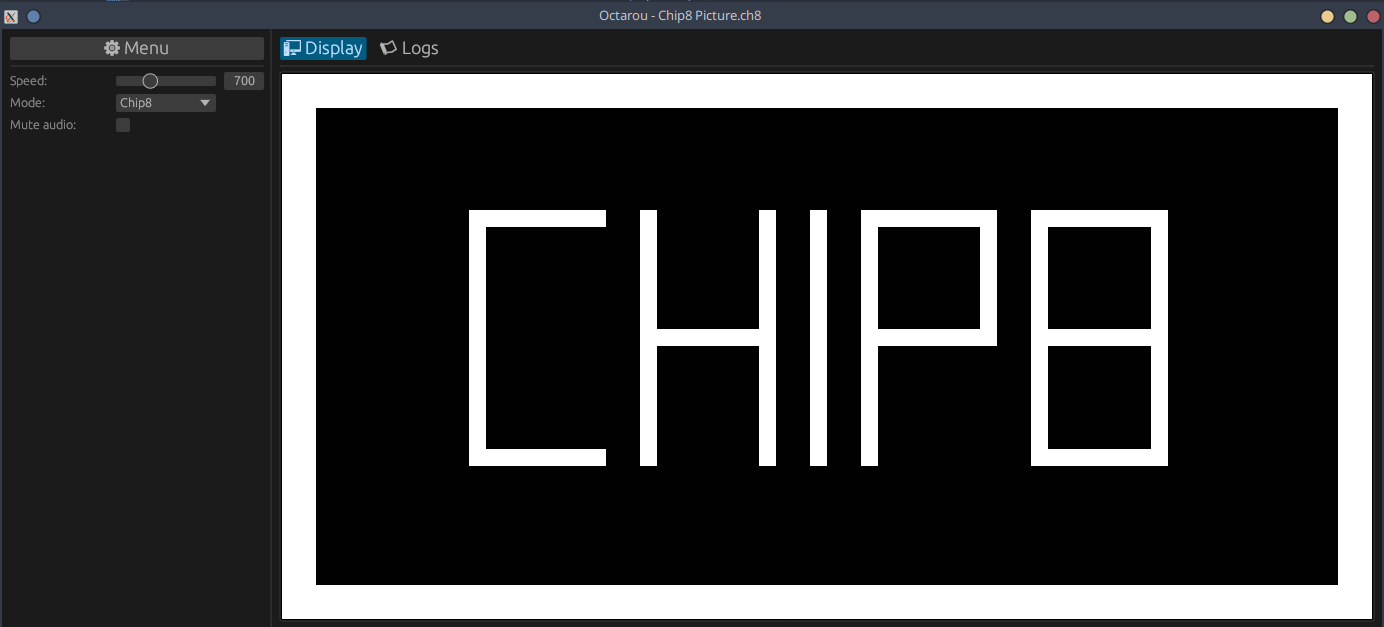
\includegraphics[width=\textwidth]{figures/chip8-logo.png}
	\end{center}
	\caption{\textit{Octarou} rulând un program simplu}
\end{figure}

\begin{figure}[p!]
	\begin{center}
		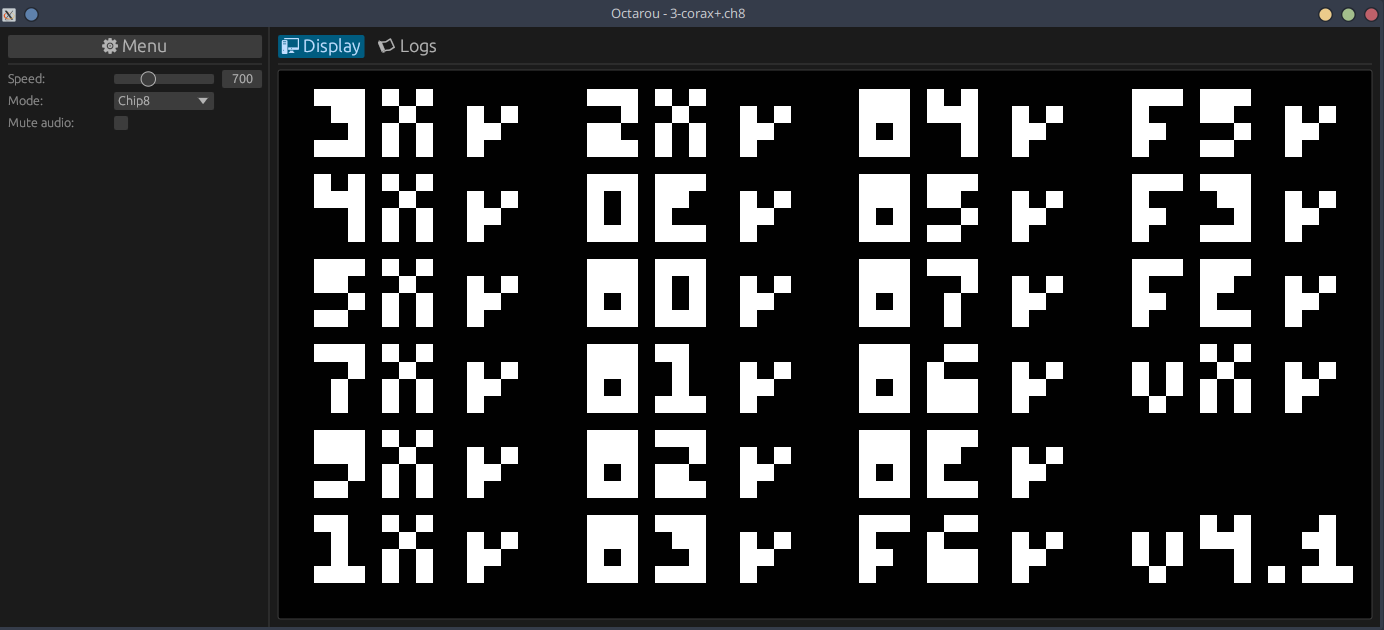
\includegraphics[width=0.95\textwidth]{figures/corax.png}
	\end{center}
	\caption{\textit{Octarou} rulând testele \texttt{corax+}}
\end{figure}

\begin{figure}[p!]
	\begin{center}
		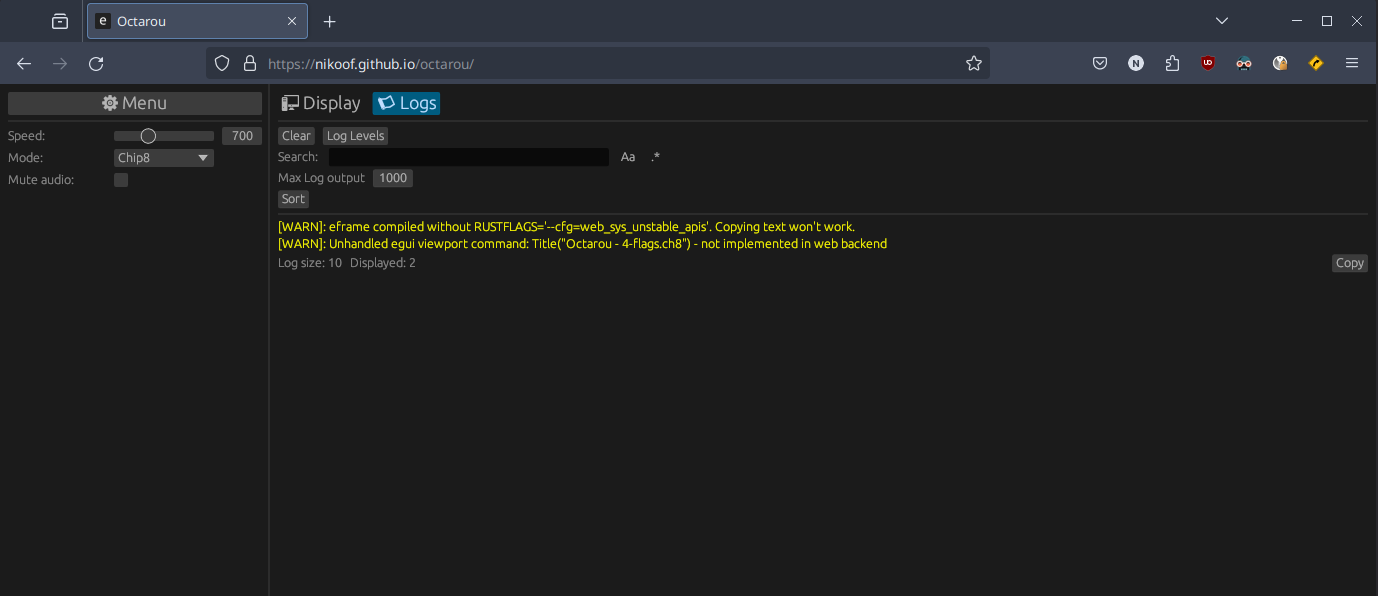
\includegraphics[width=0.95\textwidth]{figures/web.png}
	\end{center}
	\caption{Lista cu mesaje de logging a \textit{Octarou}, rulând în Mozilla Firefox}
\end{figure}

\begin{figure}[p!]
	\begin{center}
		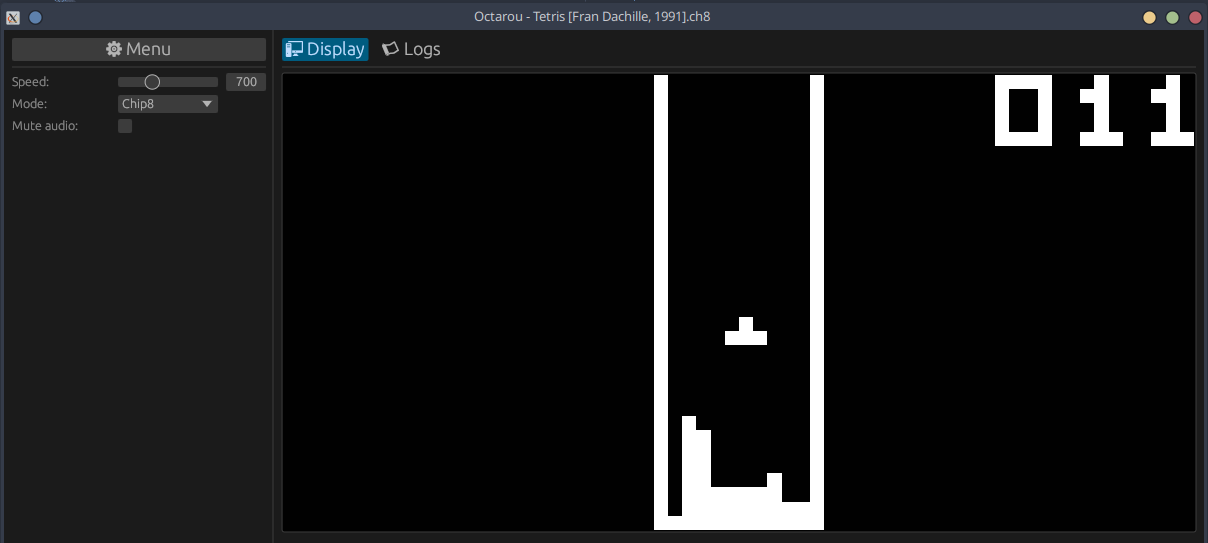
\includegraphics[width=0.95\textwidth]{figures/tetris.png}
	\end{center}
	\caption{\textit{Octarou}, rulând în faimosul joc \textit{Tetris}}
\end{figure}


%--------------------------------------------------------------------------------------------------------------------------------------------------------------%
\section{Îmbunătățiri}
Una din primele îmbunătățiri pe care aș vrea să le implementez este suportul pentru \texttt{XO-CHIP}, o variantă modernă de \texttt{CHIP-8}
folosită în \textit{Octo}, un compilator și IDE pentru \texttt{CHIP-8}. Majoritatea programelor noi sunt scrise pentru \texttt{XO-CHIP}, ceea
ce ar însemna ca interpretorul meu ar putea rula mult mai multe programe interesante.

Un alt lucru ce trebuie îmbunătățit este suportul pentru web, întrucât, versiunea 1.1.0 nu implementează temporizarea exactă, întrucât API-urile
pentru timp nu sunt implementate complet în ecosistemul WebAssembly. De aceea, deși este funcțional, experiența de utilizator pe versiunea web a
\textit{Octarou} nu este întocmai plăcută.

În afară de acestea, mereu există opțiunea să adaug mai multe chestiuni configurabile legate de diferitele variante de \texttt{CHIP-8}.
Util ar fi și un sistem de depanare a programelor. Posibilitățile în acest sens sunt numeroase.

%--------------------------------------------------------------------------------------------------------------------------------------------------------------%
\section{Concluzii}
În procesul de creare a acestui proiect, am învățat multe lucruri despre programarea în limbajul Rust și despre arhitectura sistemelor
CHIP-8 și SUPER-CHIP. Crearea unui interpretor pentru aceste sisteme a necesitat o înțelegere profundă a funcționării lor interne, precum
și abilități solide de analiză și implementare a instrucțiunilor specifice. Am fost expus la concepte precum manipularea memoriei, interpretarea
instrucțiunilor și gestionarea stării sistemului.

Unul dintre cele mai valoroase aspecte ale procesului de dezvoltare a acestui interpretor a fost navigarea prin provocările de optimizare și
gestionare a performanței, în special în ceea ce privește ciclul de execuție al instrucțiunilor. De asemenea, am experimentat cu diverse
abordări de structurare a codului și de gestionare a dependențelor într-un mod eficient și modular. Folosind Nix, am putut crea un mediu de
dezvoltare izolat și reproductibil, care a facilitat gestionarea dependențelor și a permis implementarea fără prea mult efort a unui pipeline
de CI (\textit{continuous integration}).

De asemenea, prin lucrul la acest proiect am avut ocazia să contribui la un proiect sursă deschisă \cite{eguilog}.

Acest proiect nu numai că mi-a permis să explorez concepte avansate de programare și arhitectură de calculatoare, dar mi-a oferit și oportunitatea
de a îmi îmbunătăți abilitățile de dezvoltare software. Dezvoltarea de interpretoare și emulatoare reprezintă nu doar un
exercițiu tehnic, ci și o explorare a istoriei calculatoarelor și a fundațiilor programării, punând în lumină importanța continuă a învățării și
a evoluției în acest domeniu în continuă schimbare.
%--------------------------------------------------------------------------------------------------------------------------------------------------------------%

\newpage
\printbibliography[title=\section{Bibliografie}]

\section{Index}
\renewcommand\listoflistingscaption{Listinguri de cod sursă}
\listoflistings
\listoffigures

\end{document}
